\documentclass{article}
\usepackage{parskip}
\usepackage{amsmath}
\usepackage{graphicx}
\usepackage[margin=.6in]{geometry}
\begin{document}
\title{Assignment 1}
\author{Lariesa Janecka, 20460089}
\maketitle


\section*{Question 1}
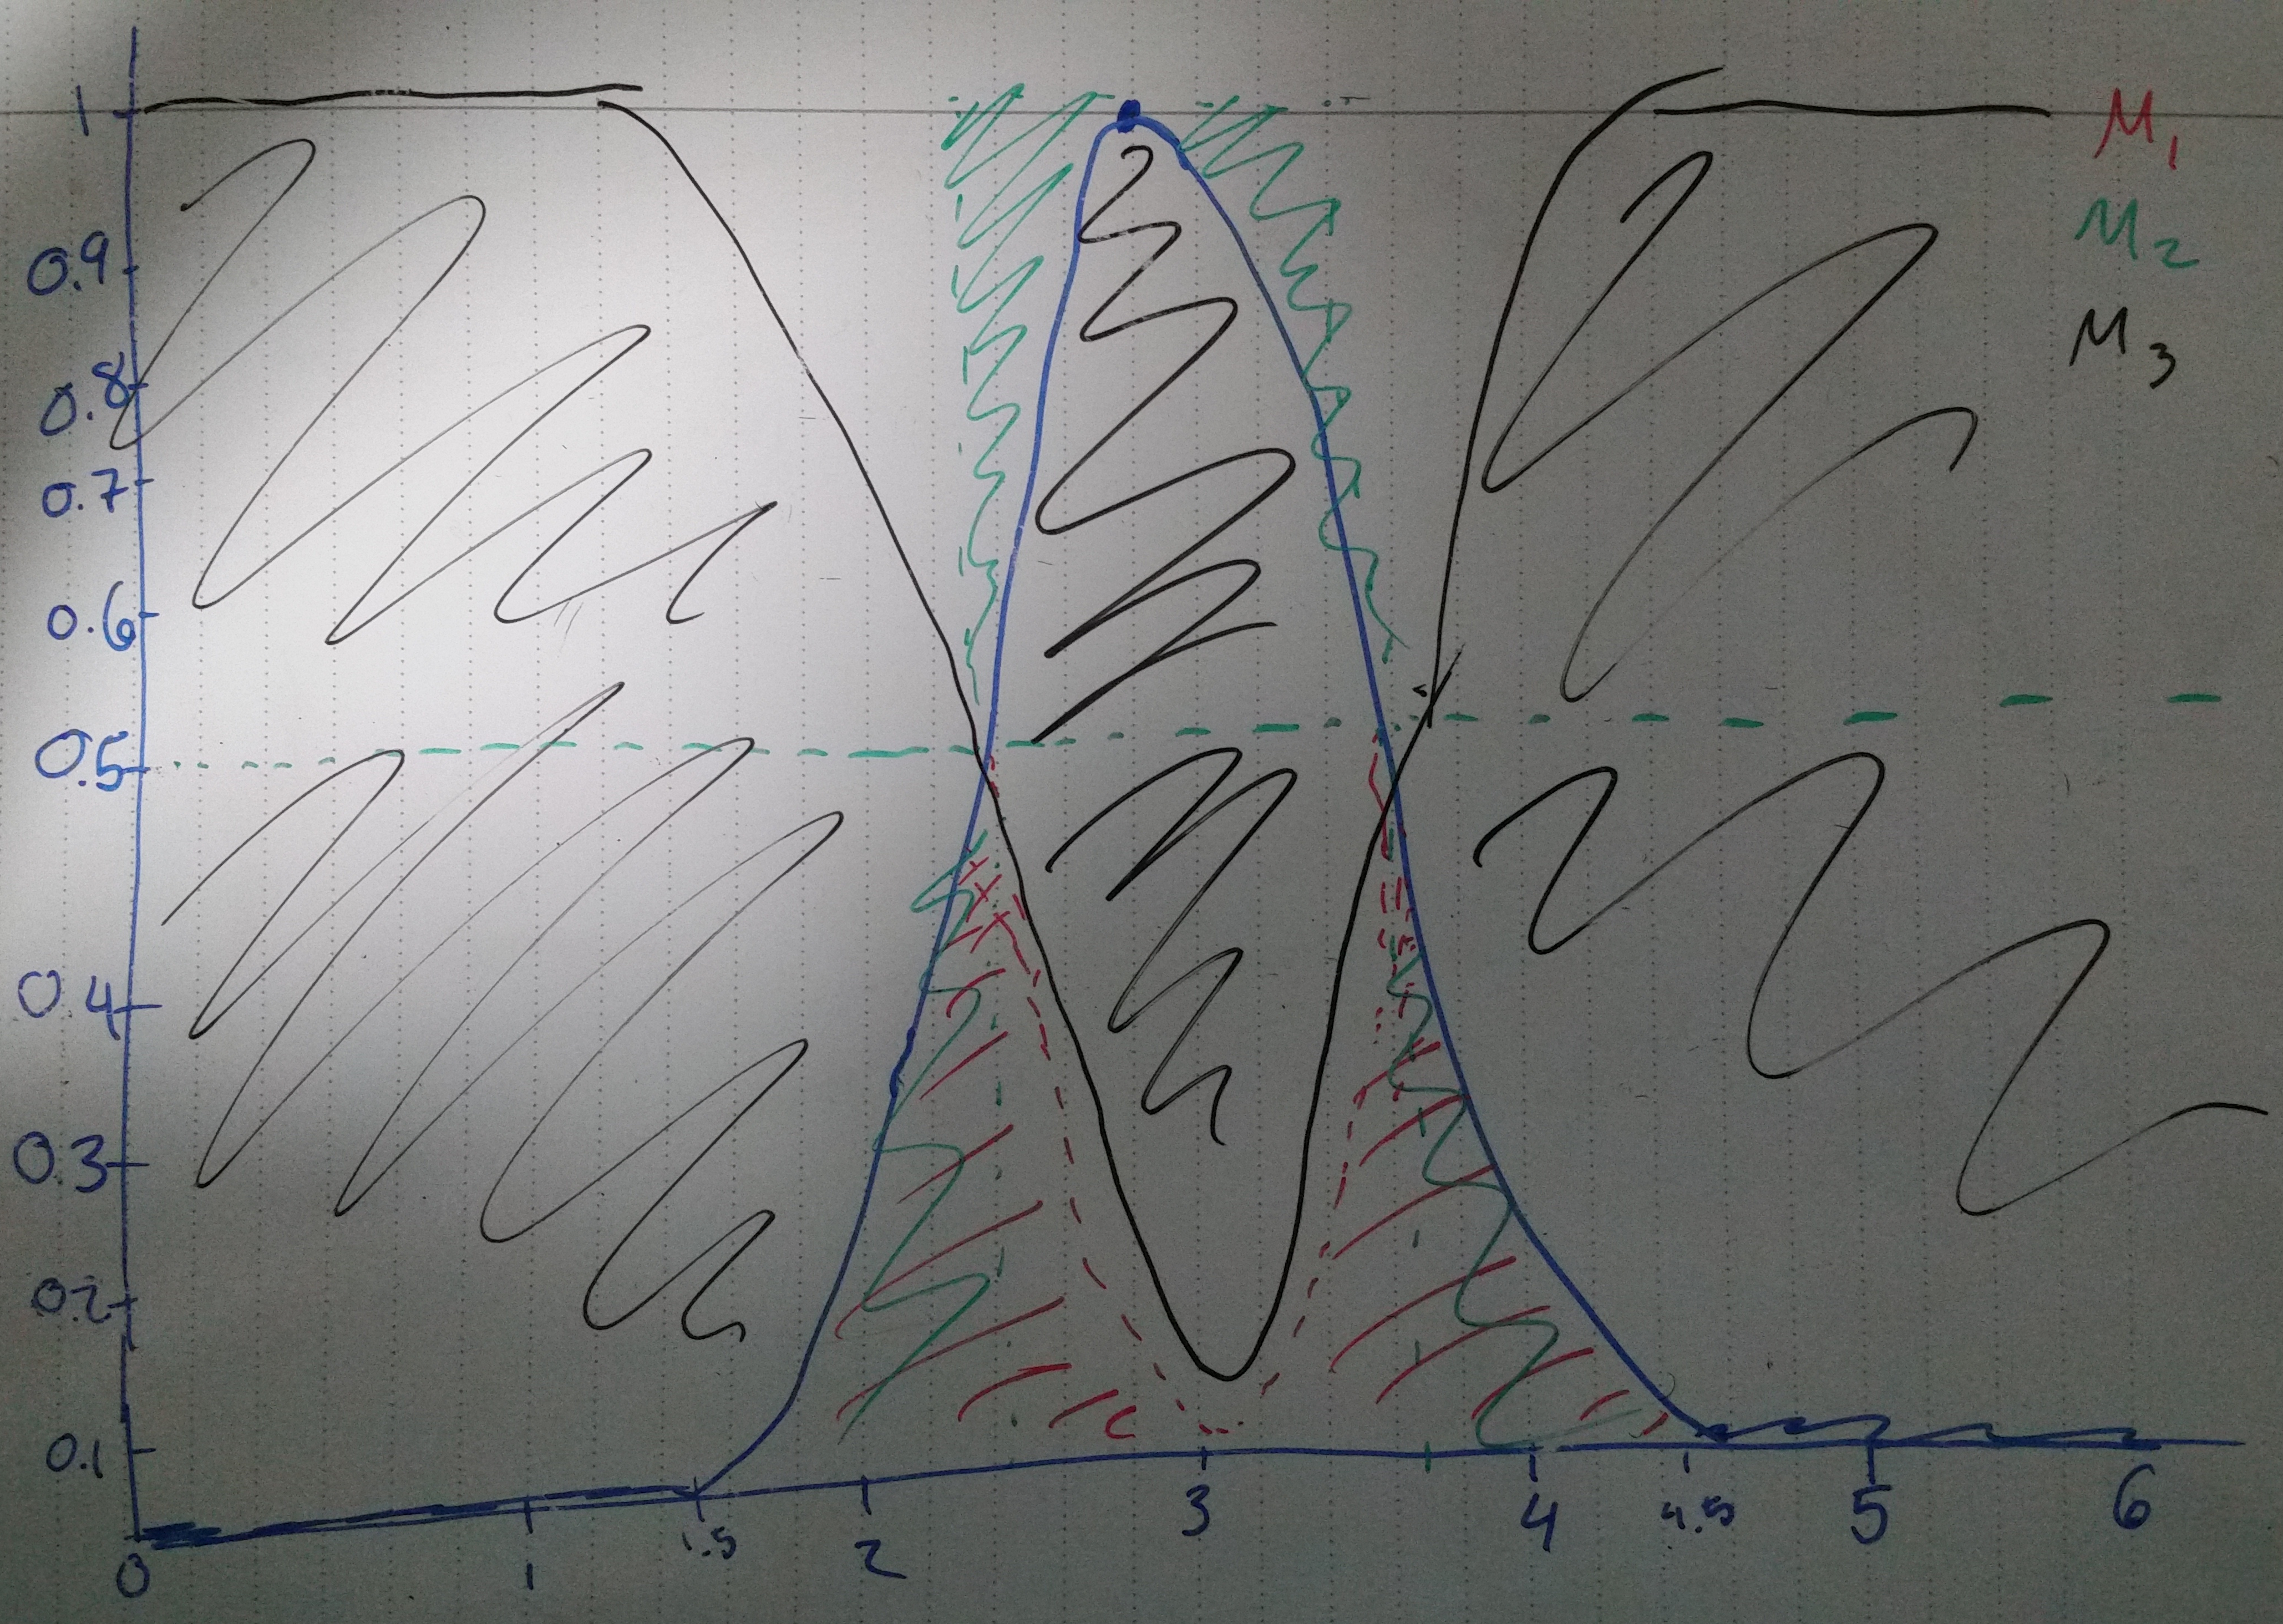
\includegraphics[width=6in]{problem1}

Note to TA: I am so sorry for my terrible art skills.

Let $S_1$ be the subset of the superset where $\mu_A(x) \leq 0.5$ and let $S_2$ be the set where $\mu_A(x) > 0.5$
\begin{align*}
	M_1 &= \int_S f(x) \text{ where } f(x) =
	\begin{cases}
	 	\mu_A(x), & \text{if } \mu_A(x) \leq 0.5\\
	 	1- \mu_A(x), &\text{otherwise}
	 \end{cases} \\
	 &= \int_{S_1} \mu_A(x) + \int_{S_2} 1-\mu_A(x)
\end{align*}
\begin{align*}
	M_2 &= \int_S |\mu_A(x) - \mu_{A_{1/2}}(x)| \text{ where } \mu_{A_{1/2}}(x) =
	\begin{cases}
		1, &\text{if } \mu_A(x) \geq 0.5\\
		0, &\text{otherwise}
	\end{cases}\\
	&= \int_{S_1}|\mu_A(x) - 0| + \int_{S_2} |\mu_A(x) - 1|\\
	&= M_1
\end{align*}
We can see that $M_1 = M_2$.



We can use these functions to measure fuzziness because they provide a way to measure the amount of uncertainty in our function. This can be thought of as the amount of space between the function and 0.5 as that is the ``center'' of the fuzziness spectrum, where it is fuzziest. This could also be thought of as the closeness to the alpha cut of 0.5 for similar reasoning of the 0.5 marker being significant. The last way is to look at the gap between the function and its compliment. The larger that gap the more fuzziness we have.

\section*{Question 2}
\[
    \chi_{A}(x)=
\begin{cases}
    1,& \text{if } x\in A\\
    0,& \text{otherwise}
\end{cases}
\]
\subsection*{a)}

If a value $x$ is in $A$ we know that it must not be in $\bar{A}$ and vice versa for values not in $A$. From this we can create a membership function.
\[
    \chi_{\bar{A}}(x)=
\begin{cases}
    0,& \text{if } \chi_{A}(x)=1\\
    1,& \text{otherwise}
\end{cases}
\]

Given that $x\in A$, then $\chi_A = 1$, and thus $\chi_{\bar{A}}(x) = 0$. So when we apply this to the equation in question:
\begin{align*}
	\chi_{\bar{A}}(x) &= 1-\chi_A(x)\\
					&= 1-1\\
					&= 0\\
					&= \chi_{\bar{A}}(x)\\
\end{align*}
Given that $x\notin A$, then $\chi_A = 0$, and thus $\chi_{\bar{A}}(x) = 1$. So when we apply this to the equation in question:
\begin{align*}
	\chi_{\bar{A}}(x) &= 1-\chi_A(x)\\
					&= 1-0\\
					&= 1\\
					&= \chi_{\bar{A}}(x)\\
\end{align*}


\subsection*{b)}
For a value to belong in the union set it must belong to at least one of the singular sets. This means that at least one of the single set membership functions must return a 1. From this we can gain a simplistic membership function.
\[
	\chi_{A\cup B}(x) =
	\begin{cases}
		1,& \text{if } \exists i | \chi_i(x) = 1 \\
		0,& \text{otherwise}
	\end{cases}
\]
By definition of max we can say that if in the set of values being considered there exists a value equal to the maximum possible value that this value will be returned. In this case the maximum value is 1 so we can define the max function for this universe as:
\begin{align*}
\max(\chi_1, \dots, \chi_n) &=
	\begin{cases}
		1,& \text{if } \exists i | \chi_i(x) = 1 \\
		0,& \text{otherwise}
	\end{cases}\\
	&= \chi_{A\cup B}(x)
\end{align*}

\subsection*{c)}
For a value to belong in the intersection set it must belong to all of the singular sets. This means that all of the single set membership functions must return a 1. From this we can gain a simplistic membership function.
\[
	\chi_{A\cap B}(x) =
	\begin{cases}
		0,& \text{if } \exists i | \chi_i(x) = 0 \\
		1,& \text{otherwise}
	\end{cases}
\]

By definition of min we can say that if in the set of values being considered there exists a value equal to the maximum possible value that this value will be returned. In this case the minimum value is 0 so we can define the min function for this universe as:
\begin{align*}
\min(\chi_1, \dots, \chi_n) &=
	\begin{cases}
		0,& \text{if } \exists i | \chi_i(x) = 0 \\
		1,& \text{otherwise}
	\end{cases}\\
	&= \chi_{A\cap B}(x)
\end{align*}

\subsubsection*{d)}
The implication operator in this case means that if $x \in A$ then it must be that $y \in B$. If $x \notin A$ then it doesn't matter what y is. This can be expanded into:
\[
	\chi_{A\rightarrow B}(x,y) =
	\begin{cases}
		\chi_B(y),& \text{if } \chi_A(x) = 1\\
		1, & \text{otherwise}
	\end{cases}
\]

\begin{align*}
	\min(1, (1-\chi_A(x) + \chi_B(y)))
	&=
	\begin{cases}
		\min(1, \chi_B(y)), & \text{if } \chi_A(x) = 1\\
		\min(1,(1 + \chi_B(y))), & \text{otherwise}\\
	\end{cases}\\
	&=
	\begin{cases}
		\chi_B(y), & \text{if } \chi_A(x) = 1\\
		1, & \text{otherwise}\\
	\end{cases}\\
	&= \chi_{A\rightarrow B}(x,y)
\end{align*}



\subsection*{e)}
These above functions are common operators used on fuzzy sets as compliment, T-norm, S-norm, and Implication functions. The fact that you can still use them on crisp sets implies that crisp sets work very similarly to fuzzy sets.


\section*{Question 3}
\subsection*{a)}
When we are applying the word ``very'' to our state we are increasing the value required to be included in the fuzzy set. This would result in less lower values included and more higher values included. If we were to imagine this on the graph of the membership function it would correspond with shifting everything right by some amount. This shift is shown in the function through subtracting some from the input, which is why the membership function of $\mu_F(v-v_0)$ is appropriate for this.

The word ``presumably'' is defined as something that is very likely. Due to this we want to narrow the range of values included in the set on both ends of the spectrum. This is exactly what the contraction operator does which is why it is appropriate here.

\subsection*{b)}
\[
	\text{Very Fast} = \left\{
		\frac{0.1}{60},
		\frac{0.3}{70},
		\frac{0.6}{80},
		\frac{0.8}{90},
		\frac{1.0}{100}
		\frac{0.7}{110}
		\frac{0.5}{120}
		\frac{0.3}{130}
		\frac{0.1}{140}
	\right\}
\]
\[
	\text{Presumably Fast} = \left\{
		\frac{0.01}{10},
		\frac{0.09}{20},
		\frac{0.36}{30},
		\frac{0.64}{40},
		\frac{1.0}{50},
		\frac{0.49}{60},
		\frac{0.25}{70},
		\frac{0.09}{80},
		\frac{0.01}{90}
	\right\}
\]

\section*{Question 4}

\subsection*{Non-decreasing}
The function can be broken into two cases.
\begin{align*}
	T(x,y) &= \max(0, x+y-1)\\
	&=
	\begin{cases}
		x+y-1, & \text{if } x+y-1 > 0 \\
		0, & \text{otherwise}
	\end{cases}
\end{align*}

Given that $a<c$ and $b<d$.

If $a+b-1 > 0$ then:
\begin{align*}
	T(a, b) &= a+b-1\\
			&< c+b-1\\
			&< c+d-1\\
			&< T(c,d)\\
\end{align*}
Since $a+b-1 > 0$ and we just proved $c+d-1 > a+b-1$ then we known $T(c, d) = c+d-1$.

If $a+b-1 \leq 0$ then $T(a,b) = 0$. Since the function is the max of 0 and some other value we know that it must return a value greater than or equal to 0 so we can say $T(c,d) \geq 0 \geq T(a,b)$.

This shows that given $a<c$ and $b<d$ then $T(a,b) \geq T(c,d)$ for all cases.

\subsection*{Commutative}
Addition is known to obey the commutative property so we can say $x+y-1 = y+x-1$.
\begin{align*}
	T(y,x) &=\max(0, y+x-1)\\
			&=\max(0, x+y-1)\\
			&=T(x,y)\\
\end{align*}
\subsection*{Associative}
Assume we have 3 values, a, b, and c.
\begin{align*}
	T(T(a,b),c) &= \max(0, \max(0, a+b-1) + c - 1)\\
	T(a,T(b,c)) &= \max(0, a + \max(0, b+c-1) - 1)\\
\end{align*}
There are two possible cases for each of the above equations, leading to four possibilities.

Assume $a+b-1 > 0$ and $b+c-1 > 0$
\begin{align*}
	T(T(a,b),c) &= \max(0, \max(0, a+b-1) + c - 1)\\
				&= \max(0, a+b-1 + c - 1)\\
				&= \max(0, a+b+c-1 - 1)\\
				&= \max(0, a+\max(0,b+c-1) - 1)\\
				&=T(T(a,b),c)
\end{align*}

Assume $a+b-1 > 0$ and $b+c-1 \leq 0$. Let $d = b+c < 1$
\begin{align*}
	T(T(a,b),c) &= \max(0, \max(0, a+b-1) + c - 1)\\
				&= \max(0, a+b-1 + c - 1)\\
				&= \max(0, a+d-2)\\
				&=0 \text{ since d and a are both less than one } a+d < 2\\
\end{align*}
\begin{align*}
	T(T(a,b),c) &= \max(0, a + \max(0, b+c-1) - 1)\\
				&= \max(0, a - 1)\\
				&= 0\\
				&=T(T(a,b),c)
\end{align*}

Assume $a+b-1 \leq 0$ and $b+c-1 > 0$. Let $d = a+b < 1$
\begin{align*}
	T(T(a,b),c) &= \max(0, \max(0, a+b-1) + c - 1)\\
				&= \max(0, c - 1)\\
				&= 0
\end{align*}
\begin{align*}
	T(a,T(b,c)) &= \max(0, a+\max(0,b+c-1) - 1)\\
				&= \max(0, a+b+c-1 - 1)\\
				&= \max(0, c+d-2)\\
				&=0 \text{ since d and c are both less than one } c+d < 2\\
				&=T(T(a,b),c)
\end{align*}

Assume $a+b-1 \leq 0$ and $b+c-1 \leq 0$.
\begin{align*}
	T(T(a,b),c) &= \max(0, \max(0, a+b-1) + c - 1)\\
				&= \max(0, c - 1)\\
				&=0
\end{align*}
\begin{align*}
	T(a,T(b,c)) &= \max(0, a+\max(0,b+c-1) - 1)\\
				&= \max(0, a- 1)\\
				&=0\\
				&=T(T(a,b),c)
\end{align*}

\subsection*{Boundary Conditions}
Let $y=1$. $T(x,1) = \max(0, x-1)$ which will equal 0 because it is impossible for x to be greater than 1.

Let $y=0$. $T(x,0) = \max(0, x)$ which will equal x because it is impossible for x to be less than 0.

\subsection*{t-conorm}
\begin{align*}
	S(x,y) &= 1-T(1-x, 1-y)\\
			&= 1-max(0, 1-x+1-y-1)\\
			&= 1-max(0, 1-x-y)\\
\end{align*}

\section*{Question 5}
\subsection*{a)}
$a$ is used to shift the center of the membership function. This would correspond to were the values that are most likely to be included in the set are located, it wouldn't affect the fuzziness of the function. We would associate this value with very if $a > 0$ or slightly if $a < 0$

$\lambda$ is used to effect the width of the membership function. This would make the function fuzzier if $\lambda > 1$ and less fuzzy if $\lambda < 1$. If $\lambda < 1$ we would use words like somehow, or more-or-less, or other such words that would include more values. If $\lambda > 1$ we would use words like mostly, or presumably, or other such words that would include less values.

$n$ is used to effect the curvature of the membership function. It will increase fuzziness as it increases and decreases with it. Many of the same words for $\lambda$ could be used here but words that express an large range of values that are more certain would apply where $n$ is increasing because it widens the top of the curve.

\subsection*{b)}
People consider room temperature to be the most comfortable and they tend to place that value between 20 and 25 degrees Celsius. These values are what will be used to set the membership functions.

People's opinion of if its hot or cold tends to drop off quickly as the temperature changes so both these functions will have $\lambda = 2$ and $n = 2$. The range of comfortable temperatures is fairly large so that function will have a $n = 3$ to reflect this plateau.

Cold:
\begin{align*}
	\mu_{cold}(x) =
	\begin{cases}
		1, & \text{if } x < 20\\
		e^{-2|x-20|^2}, & \text{otherwise}
	\end{cases}
\end{align*}

Comfortable:
\begin{align*}
	\mu_{comfy}(x) = e^{-2|x-22.5|^3}
\end{align*}

Hot:
\begin{align*}
	\mu_{hot}(x) =
	\begin{cases}
		1, & \text{if } x < 25\\
		e^{-2|x-25|^2}, & \text{otherwise}
	\end{cases}
\end{align*}


\end{document}
